\documentclass[11pt]{article}
% ---------------------------------------------------------------
% R3.07 SQL dans un langage de programmation -- preambule commun des sujets de TP
% Article clair, fond blanc, accents de couleur coherents avec les slides
% Charte derivee de R5.A.08 Qualite de developpement (meme palette IUT)
% Utilisation :
%   \documentclass[11pt]{article}
%   % ---------------------------------------------------------------
% R3.07 SQL dans un langage de programmation -- preambule commun des sujets de TP
% Article clair, fond blanc, accents de couleur coherents avec les slides
% Charte derivee de R5.A.08 Qualite de developpement (meme palette IUT)
% Utilisation :
%   \documentclass[11pt]{article}
%   % ---------------------------------------------------------------
% R3.07 SQL dans un langage de programmation -- preambule commun des sujets de TP
% Article clair, fond blanc, accents de couleur coherents avec les slides
% Charte derivee de R5.A.08 Qualite de developpement (meme palette IUT)
% Utilisation :
%   \documentclass[11pt]{article}
%   \input{../../latex/common/r307-tp-preamble.tex}
%   \begin{document}
%   \rtpheader{1}{Titre du TP}
% ---------------------------------------------------------------
\usepackage[T1]{fontenc}
\usepackage[utf8]{inputenc}
\usepackage[french]{babel}
\usepackage[scale=0.92]{tgheros}
\usepackage{tgpagella}
\usepackage[a4paper, margin=2.2cm, headheight=14pt]{geometry}
\usepackage{graphicx}
\usepackage{xcolor}
\usepackage{listings}
\usepackage[skins,listings,breakable]{tcolorbox}
\usepackage{enumitem}
\usepackage{booktabs}
\usepackage{array}
\usepackage{multirow}
\usepackage{tikz}
\usetikzlibrary{shapes, shapes.geometric, arrows, arrows.meta, positioning, calc}
\usepackage[colorlinks=true, linkcolor=qaaccentdark, urlcolor=qaaccentdark]{hyperref}
\usepackage{fancyhdr}
\usepackage{lastpage}
\usepackage{titlesec}
\usepackage{etoolbox}

% ---------------------------------------------------------------
% PALETTE -- version imprimable des couleurs des diapositives
% ---------------------------------------------------------------
\definecolor{qaaccentdark}{HTML}{7A1680}   % violet du logo IUT, fonce pour rester lisible sur blanc
\definecolor{qaaccent2dark}{HTML}{9B4B94}  % violet clair du logo IUT (accent secondaire)
\definecolor{qapanellight}{HTML}{F4F6F8}   % fond de bloc tres clair
\definecolor{qalinelight}{HTML}{D8DEE4}    % filets
\definecolor{qatextdark}{HTML}{1A1D23}     % texte principal
\definecolor{qamuteddark}{HTML}{5B6472}    % texte secondaire
\definecolor{qacodekwl}{HTML}{7A1680}      % code : mots-cles
\definecolor{qacodestrl}{HTML}{2E7D32}     % code : chaines
\definecolor{qacodecoml}{HTML}{6B7280}     % code : commentaires
\definecolor{qacodeannl}{HTML}{B26A00}     % code : annotations / javadoc

\color{qatextdark}

\setlength{\parskip}{4pt}
\setlength{\parindent}{0pt}

% ---------------------------------------------------------------
% TITRES DE SECTION -- texte blanc sur bande de couleur pleine largeur
% (gere aussi les variantes etoilees \section*)
% ---------------------------------------------------------------
\newcommand{\qasectionband}[2]{%
  \noindent\colorbox{#1}{%
    \parbox[c]{\dimexpr\linewidth-2\fboxsep\relax}{%
      \color{white}#2%
    }%
  }%
}
\newcommand{\secformat}[1]{\qasectionband{qaaccentdark}{\bfseries\Large\thesection\quad #1}}
\newcommand{\secformatnn}[1]{\qasectionband{qaaccentdark}{\bfseries\Large #1}}
\newcommand{\subsecformat}[1]{\qasectionband{qaaccent2dark}{\bfseries\large\thesubsection\quad #1}}
\newcommand{\subsecformatnn}[1]{\qasectionband{qaaccent2dark}{\bfseries\large #1}}

\titleformat{\section}{\normalfont}{}{0pt}{\secformat}
\titleformat{name=\section,numberless}{\normalfont}{}{0pt}{\secformatnn}
\titleformat{\subsection}{\normalfont}{}{0pt}{\subsecformat}
\titleformat{name=\subsection,numberless}{\normalfont}{}{0pt}{\subsecformatnn}
\titleformat{\subsubsection}{\normalfont\bfseries\color{qaaccentdark}}{\thesubsubsection}{0.6em}{}
\titlespacing*{\section}{0pt}{14pt}{8pt}
\titlespacing*{\subsection}{0pt}{10pt}{6pt}
\titlespacing*{\subsubsection}{0pt}{8pt}{4pt}

% ---------------------------------------------------------------
% LISTINGS -- theme clair (lstlisting reste utilisable tel quel)
% \lstcode : police + couleur de base, a reutiliser dans les surcharges
% ---------------------------------------------------------------
\newcommand{\lstcode}{\ttfamily\color{qatextdark}}

\lstdefinelanguage{TypeScript}{
  keywords={typeof, new, true, false, catch, function, return, null, switch, var,
    if, in, while, do, else, case, break, const, let, interface, class, extends,
    implements, enum, export, import, this, super, constructor, public, private,
    protected, static, async, await, throw, throws, try, finally, void},
  ndkeywords={boolean, any, number, string, int, long, double},
  sensitive=true,
  comment=[l]{//},
  morecomment=[s]{/*}{*/},
  morestring=[b]',
  morestring=[b]"
}

\lstdefinestyle{r307code}{
  basicstyle=\lstcode\footnotesize,
  keywordstyle=\color{qacodekwl}\bfseries,
  ndkeywordstyle=\color{qaaccent2dark}\bfseries,
  stringstyle=\color{qacodestrl},
  commentstyle=\color{qacodecoml}\itshape,
  morecomment=[s][\color{qacodeannl}]{/**}{*/},
  backgroundcolor=\color{qapanellight},
  rulecolor=\color{qalinelight},
  frame=single,
  framesep=4pt,
  xleftmargin=6pt,
  xrightmargin=6pt,
  numbers=left,
  numberstyle=\tiny\color{qamuteddark},
  numbersep=8pt,
  keepspaces=true,
  columns=fullflexible,
  showstringspaces=false,
  showspaces=false,
  showtabs=false,
  breaklines=true,
  breakatwhitespace=false,
  captionpos=b,
  tabsize=2,
  escapeinside={(*@}{@*)},
}
\lstset{style=r307code}

% ---------------------------------------------------------------
% BOITES : exercice, code, information
% ---------------------------------------------------------------
\tcbset{
  exobox/.style={colback=qapanellight, colframe=qaaccentdark, boxrule=0.6pt,
    arc=2pt, left=8pt, right=8pt, top=6pt, bottom=6pt,
    coltitle=white, colbacktitle=qaaccentdark, fonttitle=\bfseries,
    boxsep=2pt, breakable},
  infobox/.style={colback=white, colframe=qaaccent2dark, boxrule=0.6pt,
    leftrule=3pt, arc=0pt, left=8pt, right=8pt, top=5pt, bottom=5pt,
    coltitle=qaaccent2dark, colbacktitle=white, fonttitle=\bfseries,
    breakable},
  codebox/.style={colback=qatextdark, colframe=qalinelight, boxrule=0.4pt,
    arc=2pt, left=8pt, right=8pt, top=5pt, bottom=5pt, listing only,
    listing options={basicstyle=\ttfamily\small\color{white},
      breaklines=true, showstringspaces=false, columns=fullflexible,
      keepspaces=true, frame=none, numbers=none, backgroundcolor={}}, breakable}
}
\newtcolorbox[auto counter]{exobox}[2][]{exobox,
  title={Exercice~\thetcbcounter\ifstrempty{#2}{}{ --- #2}}, #1}
\newtcolorbox{infobox}[1][\`A retenir]{infobox, title={#1}}
\newtcblisting{codebox}{codebox}

% ---------------------------------------------------------------
% EN-TETE DE PAGE (fil d'Ariane + pagination)
% ---------------------------------------------------------------
\newcommand{\qaheadtitlevalue}{}
\newcommand{\qaheadtitle}[1]{\renewcommand{\qaheadtitlevalue}{#1}}

\pagestyle{fancy}
\fancyhf{}
\renewcommand{\headrulewidth}{0.4pt}
\fancyhead[L]{\small\color{qamuteddark}R3.07 --- \qaheadtitlevalue}
\fancyhead[R]{\small\color{qamuteddark}\thepage\,/\,\pageref{LastPage}}
\fancyfoot[C]{\footnotesize\color{qamuteddark}IUT de Vannes --- Universit\'e Bretagne Sud}
\fancypagestyle{plain}{\fancyhf{}\renewcommand{\headrulewidth}{0pt}%
  \fancyfoot[C]{\footnotesize\color{qamuteddark}IUT de Vannes --- Universit\'e Bretagne Sud}}

% ---------------------------------------------------------------
% BANDEAU DE TITRE (pas une page dediee, pour rester compact)
% \rtpheader{numero ou intitule court}{titre du TP}
% ---------------------------------------------------------------
\newcommand{\ryear}{2026/2027}
\newcommand{\rtpheader}[2]{%
  \thispagestyle{plain}%
  \begin{minipage}[t]{0.68\textwidth}
    {\small\color{qamuteddark}
      Universit\'e Bretagne Sud\\
      IUT de Vannes\\
      D\'epartement Informatique --- \ryear}
  \end{minipage}%
  \hfill
  \begin{minipage}[t]{0.28\textwidth}
    \raggedleft
    \includegraphics[width=2.6cm]{iut_logo.jpg}
  \end{minipage}

  \vspace{6mm}
  \begin{center}
    {\large\bfseries\color{qatextdark} BUT 2 --- R3.07. SQL dans un langage de programmation}\\[2mm]
    {\normalsize\color{qamuteddark} TD/TP #1}\\[1mm]
    {\Large\bfseries\color{qaaccentdark} #2}
  \end{center}
  \vspace{4mm}
  \qaheadtitle{#2}
}

%   \begin{document}
%   \rtpheader{1}{Titre du TP}
% ---------------------------------------------------------------
\usepackage[T1]{fontenc}
\usepackage[utf8]{inputenc}
\usepackage[french]{babel}
\usepackage[scale=0.92]{tgheros}
\usepackage{tgpagella}
\usepackage[a4paper, margin=2.2cm, headheight=14pt]{geometry}
\usepackage{graphicx}
\usepackage{xcolor}
\usepackage{listings}
\usepackage[skins,listings,breakable]{tcolorbox}
\usepackage{enumitem}
\usepackage{booktabs}
\usepackage{array}
\usepackage{multirow}
\usepackage{tikz}
\usetikzlibrary{shapes, shapes.geometric, arrows, arrows.meta, positioning, calc}
\usepackage[colorlinks=true, linkcolor=qaaccentdark, urlcolor=qaaccentdark]{hyperref}
\usepackage{fancyhdr}
\usepackage{lastpage}
\usepackage{titlesec}
\usepackage{etoolbox}

% ---------------------------------------------------------------
% PALETTE -- version imprimable des couleurs des diapositives
% ---------------------------------------------------------------
\definecolor{qaaccentdark}{HTML}{7A1680}   % violet du logo IUT, fonce pour rester lisible sur blanc
\definecolor{qaaccent2dark}{HTML}{9B4B94}  % violet clair du logo IUT (accent secondaire)
\definecolor{qapanellight}{HTML}{F4F6F8}   % fond de bloc tres clair
\definecolor{qalinelight}{HTML}{D8DEE4}    % filets
\definecolor{qatextdark}{HTML}{1A1D23}     % texte principal
\definecolor{qamuteddark}{HTML}{5B6472}    % texte secondaire
\definecolor{qacodekwl}{HTML}{7A1680}      % code : mots-cles
\definecolor{qacodestrl}{HTML}{2E7D32}     % code : chaines
\definecolor{qacodecoml}{HTML}{6B7280}     % code : commentaires
\definecolor{qacodeannl}{HTML}{B26A00}     % code : annotations / javadoc

\color{qatextdark}

\setlength{\parskip}{4pt}
\setlength{\parindent}{0pt}

% ---------------------------------------------------------------
% TITRES DE SECTION -- texte blanc sur bande de couleur pleine largeur
% (gere aussi les variantes etoilees \section*)
% ---------------------------------------------------------------
\newcommand{\qasectionband}[2]{%
  \noindent\colorbox{#1}{%
    \parbox[c]{\dimexpr\linewidth-2\fboxsep\relax}{%
      \color{white}#2%
    }%
  }%
}
\newcommand{\secformat}[1]{\qasectionband{qaaccentdark}{\bfseries\Large\thesection\quad #1}}
\newcommand{\secformatnn}[1]{\qasectionband{qaaccentdark}{\bfseries\Large #1}}
\newcommand{\subsecformat}[1]{\qasectionband{qaaccent2dark}{\bfseries\large\thesubsection\quad #1}}
\newcommand{\subsecformatnn}[1]{\qasectionband{qaaccent2dark}{\bfseries\large #1}}

\titleformat{\section}{\normalfont}{}{0pt}{\secformat}
\titleformat{name=\section,numberless}{\normalfont}{}{0pt}{\secformatnn}
\titleformat{\subsection}{\normalfont}{}{0pt}{\subsecformat}
\titleformat{name=\subsection,numberless}{\normalfont}{}{0pt}{\subsecformatnn}
\titleformat{\subsubsection}{\normalfont\bfseries\color{qaaccentdark}}{\thesubsubsection}{0.6em}{}
\titlespacing*{\section}{0pt}{14pt}{8pt}
\titlespacing*{\subsection}{0pt}{10pt}{6pt}
\titlespacing*{\subsubsection}{0pt}{8pt}{4pt}

% ---------------------------------------------------------------
% LISTINGS -- theme clair (lstlisting reste utilisable tel quel)
% \lstcode : police + couleur de base, a reutiliser dans les surcharges
% ---------------------------------------------------------------
\newcommand{\lstcode}{\ttfamily\color{qatextdark}}

\lstdefinelanguage{TypeScript}{
  keywords={typeof, new, true, false, catch, function, return, null, switch, var,
    if, in, while, do, else, case, break, const, let, interface, class, extends,
    implements, enum, export, import, this, super, constructor, public, private,
    protected, static, async, await, throw, throws, try, finally, void},
  ndkeywords={boolean, any, number, string, int, long, double},
  sensitive=true,
  comment=[l]{//},
  morecomment=[s]{/*}{*/},
  morestring=[b]',
  morestring=[b]"
}

\lstdefinestyle{r307code}{
  basicstyle=\lstcode\footnotesize,
  keywordstyle=\color{qacodekwl}\bfseries,
  ndkeywordstyle=\color{qaaccent2dark}\bfseries,
  stringstyle=\color{qacodestrl},
  commentstyle=\color{qacodecoml}\itshape,
  morecomment=[s][\color{qacodeannl}]{/**}{*/},
  backgroundcolor=\color{qapanellight},
  rulecolor=\color{qalinelight},
  frame=single,
  framesep=4pt,
  xleftmargin=6pt,
  xrightmargin=6pt,
  numbers=left,
  numberstyle=\tiny\color{qamuteddark},
  numbersep=8pt,
  keepspaces=true,
  columns=fullflexible,
  showstringspaces=false,
  showspaces=false,
  showtabs=false,
  breaklines=true,
  breakatwhitespace=false,
  captionpos=b,
  tabsize=2,
  escapeinside={(*@}{@*)},
}
\lstset{style=r307code}

% ---------------------------------------------------------------
% BOITES : exercice, code, information
% ---------------------------------------------------------------
\tcbset{
  exobox/.style={colback=qapanellight, colframe=qaaccentdark, boxrule=0.6pt,
    arc=2pt, left=8pt, right=8pt, top=6pt, bottom=6pt,
    coltitle=white, colbacktitle=qaaccentdark, fonttitle=\bfseries,
    boxsep=2pt, breakable},
  infobox/.style={colback=white, colframe=qaaccent2dark, boxrule=0.6pt,
    leftrule=3pt, arc=0pt, left=8pt, right=8pt, top=5pt, bottom=5pt,
    coltitle=qaaccent2dark, colbacktitle=white, fonttitle=\bfseries,
    breakable},
  codebox/.style={colback=qatextdark, colframe=qalinelight, boxrule=0.4pt,
    arc=2pt, left=8pt, right=8pt, top=5pt, bottom=5pt, listing only,
    listing options={basicstyle=\ttfamily\small\color{white},
      breaklines=true, showstringspaces=false, columns=fullflexible,
      keepspaces=true, frame=none, numbers=none, backgroundcolor={}}, breakable}
}
\newtcolorbox[auto counter]{exobox}[2][]{exobox,
  title={Exercice~\thetcbcounter\ifstrempty{#2}{}{ --- #2}}, #1}
\newtcolorbox{infobox}[1][\`A retenir]{infobox, title={#1}}
\newtcblisting{codebox}{codebox}

% ---------------------------------------------------------------
% EN-TETE DE PAGE (fil d'Ariane + pagination)
% ---------------------------------------------------------------
\newcommand{\qaheadtitlevalue}{}
\newcommand{\qaheadtitle}[1]{\renewcommand{\qaheadtitlevalue}{#1}}

\pagestyle{fancy}
\fancyhf{}
\renewcommand{\headrulewidth}{0.4pt}
\fancyhead[L]{\small\color{qamuteddark}R3.07 --- \qaheadtitlevalue}
\fancyhead[R]{\small\color{qamuteddark}\thepage\,/\,\pageref{LastPage}}
\fancyfoot[C]{\footnotesize\color{qamuteddark}IUT de Vannes --- Universit\'e Bretagne Sud}
\fancypagestyle{plain}{\fancyhf{}\renewcommand{\headrulewidth}{0pt}%
  \fancyfoot[C]{\footnotesize\color{qamuteddark}IUT de Vannes --- Universit\'e Bretagne Sud}}

% ---------------------------------------------------------------
% BANDEAU DE TITRE (pas une page dediee, pour rester compact)
% \rtpheader{numero ou intitule court}{titre du TP}
% ---------------------------------------------------------------
\newcommand{\ryear}{2026/2027}
\newcommand{\rtpheader}[2]{%
  \thispagestyle{plain}%
  \begin{minipage}[t]{0.68\textwidth}
    {\small\color{qamuteddark}
      Universit\'e Bretagne Sud\\
      IUT de Vannes\\
      D\'epartement Informatique --- \ryear}
  \end{minipage}%
  \hfill
  \begin{minipage}[t]{0.28\textwidth}
    \raggedleft
    \includegraphics[width=2.6cm]{iut_logo.jpg}
  \end{minipage}

  \vspace{6mm}
  \begin{center}
    {\large\bfseries\color{qatextdark} BUT 2 --- R3.07. SQL dans un langage de programmation}\\[2mm]
    {\normalsize\color{qamuteddark} TD/TP #1}\\[1mm]
    {\Large\bfseries\color{qaaccentdark} #2}
  \end{center}
  \vspace{4mm}
  \qaheadtitle{#2}
}

%   \begin{document}
%   \rtpheader{1}{Titre du TP}
% ---------------------------------------------------------------
\usepackage[T1]{fontenc}
\usepackage[utf8]{inputenc}
\usepackage[french]{babel}
\usepackage[scale=0.92]{tgheros}
\usepackage{tgpagella}
\usepackage[a4paper, margin=2.2cm, headheight=14pt]{geometry}
\usepackage{graphicx}
\usepackage{xcolor}
\usepackage{listings}
\usepackage[skins,listings,breakable]{tcolorbox}
\usepackage{enumitem}
\usepackage{booktabs}
\usepackage{array}
\usepackage{multirow}
\usepackage{tikz}
\usetikzlibrary{shapes, shapes.geometric, arrows, arrows.meta, positioning, calc}
\usepackage[colorlinks=true, linkcolor=qaaccentdark, urlcolor=qaaccentdark]{hyperref}
\usepackage{fancyhdr}
\usepackage{lastpage}
\usepackage{titlesec}
\usepackage{etoolbox}

% ---------------------------------------------------------------
% PALETTE -- version imprimable des couleurs des diapositives
% ---------------------------------------------------------------
\definecolor{qaaccentdark}{HTML}{7A1680}   % violet du logo IUT, fonce pour rester lisible sur blanc
\definecolor{qaaccent2dark}{HTML}{9B4B94}  % violet clair du logo IUT (accent secondaire)
\definecolor{qapanellight}{HTML}{F4F6F8}   % fond de bloc tres clair
\definecolor{qalinelight}{HTML}{D8DEE4}    % filets
\definecolor{qatextdark}{HTML}{1A1D23}     % texte principal
\definecolor{qamuteddark}{HTML}{5B6472}    % texte secondaire
\definecolor{qacodekwl}{HTML}{7A1680}      % code : mots-cles
\definecolor{qacodestrl}{HTML}{2E7D32}     % code : chaines
\definecolor{qacodecoml}{HTML}{6B7280}     % code : commentaires
\definecolor{qacodeannl}{HTML}{B26A00}     % code : annotations / javadoc

\color{qatextdark}

\setlength{\parskip}{4pt}
\setlength{\parindent}{0pt}

% ---------------------------------------------------------------
% TITRES DE SECTION -- texte blanc sur bande de couleur pleine largeur
% (gere aussi les variantes etoilees \section*)
% ---------------------------------------------------------------
\newcommand{\qasectionband}[2]{%
  \noindent\colorbox{#1}{%
    \parbox[c]{\dimexpr\linewidth-2\fboxsep\relax}{%
      \color{white}#2%
    }%
  }%
}
\newcommand{\secformat}[1]{\qasectionband{qaaccentdark}{\bfseries\Large\thesection\quad #1}}
\newcommand{\secformatnn}[1]{\qasectionband{qaaccentdark}{\bfseries\Large #1}}
\newcommand{\subsecformat}[1]{\qasectionband{qaaccent2dark}{\bfseries\large\thesubsection\quad #1}}
\newcommand{\subsecformatnn}[1]{\qasectionband{qaaccent2dark}{\bfseries\large #1}}

\titleformat{\section}{\normalfont}{}{0pt}{\secformat}
\titleformat{name=\section,numberless}{\normalfont}{}{0pt}{\secformatnn}
\titleformat{\subsection}{\normalfont}{}{0pt}{\subsecformat}
\titleformat{name=\subsection,numberless}{\normalfont}{}{0pt}{\subsecformatnn}
\titleformat{\subsubsection}{\normalfont\bfseries\color{qaaccentdark}}{\thesubsubsection}{0.6em}{}
\titlespacing*{\section}{0pt}{14pt}{8pt}
\titlespacing*{\subsection}{0pt}{10pt}{6pt}
\titlespacing*{\subsubsection}{0pt}{8pt}{4pt}

% ---------------------------------------------------------------
% LISTINGS -- theme clair (lstlisting reste utilisable tel quel)
% \lstcode : police + couleur de base, a reutiliser dans les surcharges
% ---------------------------------------------------------------
\newcommand{\lstcode}{\ttfamily\color{qatextdark}}

\lstdefinelanguage{TypeScript}{
  keywords={typeof, new, true, false, catch, function, return, null, switch, var,
    if, in, while, do, else, case, break, const, let, interface, class, extends,
    implements, enum, export, import, this, super, constructor, public, private,
    protected, static, async, await, throw, throws, try, finally, void},
  ndkeywords={boolean, any, number, string, int, long, double},
  sensitive=true,
  comment=[l]{//},
  morecomment=[s]{/*}{*/},
  morestring=[b]',
  morestring=[b]"
}

\lstdefinestyle{r307code}{
  basicstyle=\lstcode\footnotesize,
  keywordstyle=\color{qacodekwl}\bfseries,
  ndkeywordstyle=\color{qaaccent2dark}\bfseries,
  stringstyle=\color{qacodestrl},
  commentstyle=\color{qacodecoml}\itshape,
  morecomment=[s][\color{qacodeannl}]{/**}{*/},
  backgroundcolor=\color{qapanellight},
  rulecolor=\color{qalinelight},
  frame=single,
  framesep=4pt,
  xleftmargin=6pt,
  xrightmargin=6pt,
  numbers=left,
  numberstyle=\tiny\color{qamuteddark},
  numbersep=8pt,
  keepspaces=true,
  columns=fullflexible,
  showstringspaces=false,
  showspaces=false,
  showtabs=false,
  breaklines=true,
  breakatwhitespace=false,
  captionpos=b,
  tabsize=2,
  escapeinside={(*@}{@*)},
}
\lstset{style=r307code}

% ---------------------------------------------------------------
% BOITES : exercice, code, information
% ---------------------------------------------------------------
\tcbset{
  exobox/.style={colback=qapanellight, colframe=qaaccentdark, boxrule=0.6pt,
    arc=2pt, left=8pt, right=8pt, top=6pt, bottom=6pt,
    coltitle=white, colbacktitle=qaaccentdark, fonttitle=\bfseries,
    boxsep=2pt, breakable},
  infobox/.style={colback=white, colframe=qaaccent2dark, boxrule=0.6pt,
    leftrule=3pt, arc=0pt, left=8pt, right=8pt, top=5pt, bottom=5pt,
    coltitle=qaaccent2dark, colbacktitle=white, fonttitle=\bfseries,
    breakable},
  codebox/.style={colback=qatextdark, colframe=qalinelight, boxrule=0.4pt,
    arc=2pt, left=8pt, right=8pt, top=5pt, bottom=5pt, listing only,
    listing options={basicstyle=\ttfamily\small\color{white},
      breaklines=true, showstringspaces=false, columns=fullflexible,
      keepspaces=true, frame=none, numbers=none, backgroundcolor={}}, breakable}
}
\newtcolorbox[auto counter]{exobox}[2][]{exobox,
  title={Exercice~\thetcbcounter\ifstrempty{#2}{}{ --- #2}}, #1}
\newtcolorbox{infobox}[1][\`A retenir]{infobox, title={#1}}
\newtcblisting{codebox}{codebox}

% ---------------------------------------------------------------
% EN-TETE DE PAGE (fil d'Ariane + pagination)
% ---------------------------------------------------------------
\newcommand{\qaheadtitlevalue}{}
\newcommand{\qaheadtitle}[1]{\renewcommand{\qaheadtitlevalue}{#1}}

\pagestyle{fancy}
\fancyhf{}
\renewcommand{\headrulewidth}{0.4pt}
\fancyhead[L]{\small\color{qamuteddark}R3.07 --- \qaheadtitlevalue}
\fancyhead[R]{\small\color{qamuteddark}\thepage\,/\,\pageref{LastPage}}
\fancyfoot[C]{\footnotesize\color{qamuteddark}IUT de Vannes --- Universit\'e Bretagne Sud}
\fancypagestyle{plain}{\fancyhf{}\renewcommand{\headrulewidth}{0pt}%
  \fancyfoot[C]{\footnotesize\color{qamuteddark}IUT de Vannes --- Universit\'e Bretagne Sud}}

% ---------------------------------------------------------------
% BANDEAU DE TITRE (pas une page dediee, pour rester compact)
% \rtpheader{numero ou intitule court}{titre du TP}
% ---------------------------------------------------------------
\newcommand{\ryear}{2026/2027}
\newcommand{\rtpheader}[2]{%
  \thispagestyle{plain}%
  \begin{minipage}[t]{0.68\textwidth}
    {\small\color{qamuteddark}
      Universit\'e Bretagne Sud\\
      IUT de Vannes\\
      D\'epartement Informatique --- \ryear}
  \end{minipage}%
  \hfill
  \begin{minipage}[t]{0.28\textwidth}
    \raggedleft
    \includegraphics[width=2.6cm]{iut_logo.jpg}
  \end{minipage}

  \vspace{6mm}
  \begin{center}
    {\large\bfseries\color{qatextdark} BUT 2 --- R3.07. SQL dans un langage de programmation}\\[2mm]
    {\normalsize\color{qamuteddark} TD/TP #1}\\[1mm]
    {\Large\bfseries\color{qaaccentdark} #2}
  \end{center}
  \vspace{4mm}
  \qaheadtitle{#2}
}

\graphicspath{{../../latex/common/assets/}{./}}


\begin{document}
\rtpheader{2}{Approfondissement JDBC et bonnes pratiques}


\section{Introduction}
Dans ce TP, vous allez approfondir l’utilisation de JDBC en ajoutant des contraintes utiles à votre base de données, en sécurisant les informations sensibles avec un fichier \texttt{.env}, et en implémentant une classe associative pour modéliser la relation entre \texttt{Compte} et \texttt{Client}. Vous apprendrez également à réaliser des \texttt{INSERT} propres en utilisant des transactions et la gestion d’exceptions.

\section{Prérequis}
\begin{itemize}
    \item Avoir terminé le TP précédent (JDBC et Docker).
    \item Connaître les bases des transactions SQL.
    \item Savoir utiliser les exceptions en Java.
\end{itemize}

\section{Diagramme de la base de données}
\begin{center}
    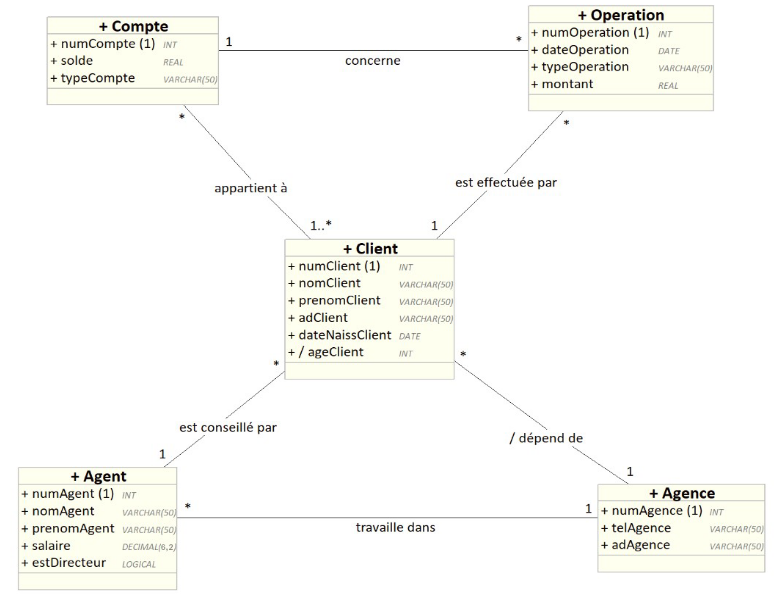
\includegraphics[width=1\textwidth]{img/db_schema.png}
\end{center}
\textit{Note : Une nouvelle table \texttt{Compte\_Client} doit être ajoutée pour modéliser la relation entre \texttt{Compte} et \texttt{Client}.}

\section{Description des nouvelles contraintes et tables}
\subsection{Contraintes à ajouter}
Vous allez modifier le schéma de la base de données en ajoutant les contraintes suivantes :
\begin{itemize}
    \item \texttt{NOT NULL} sur les colonnes obligatoires.
    \item \texttt{CHECK} sur \texttt{ageClient}, \texttt{solde}, \texttt{montant}, \texttt{salaire}.
    \item \texttt{DEFAULT} pour \texttt{estDirecteur} (valeur par défaut : \texttt{false}).
    \item \texttt{UNIQUE} pour \texttt{telAgence}.
\end{itemize}
Ces contraintes seront ajoutées via des requêtes \texttt{ALTER TABLE}, ce qui permet de modifier le schéma sans tout recréer.

\subsection{Classe associative \texttt{Compte\_Client}}
Cette table permettra de gérer la relation plusieurs-à-plusieurs entre \texttt{Compte} et \texttt{Client} :
\begin{lstlisting}[language=SQL,breaklines=true]
CREATE TABLE IF NOT EXISTS Compte_Client (
    numCompte INT REFERENCES Compte(numCompte),
    numClient INT REFERENCES Client(numClient),
    PRIMARY KEY (numCompte, numClient)
);
\end{lstlisting}

\section{Mise à jour de la base de données}
\subsection{Étape 1 : Ajouter les contraintes avec \texttt{ALTER TABLE}}
Modifiez le fichier \texttt{init.sql} pour ajouter les contraintes après la création des tables :
\begin{lstlisting}[language=SQL,breaklines=true]
-- Exemple pour la table Client
ALTER TABLE Client
    ALTER COLUMN nomClient SET NOT NULL,
    ALTER COLUMN prenomClient SET NOT NULL,
    ADD CONSTRAINT chk_age CHECK (ageClient >= 18);

-- Exemple pour la table Compte
ALTER TABLE Compte
    ADD CONSTRAINT chk_solde CHECK (solde >= 0);

-- Exemple pour la table Agence
ALTER TABLE Agence
    ADD CONSTRAINT unique_telAgence UNIQUE (telAgence);

-- Exemple pour la table Agent
ALTER TABLE Agent
    ALTER COLUMN estDirecteur SET DEFAULT false;
\end{lstlisting}
\textit{Grace à cette écriture différentielle on modifie uniquement ce qui change, ce qui est plus maintenable et moins risqué.}

\subsection{Étape 2 : Créer un fichier \texttt{.env}}
Pour sécuriser les informations sensibles, créez un fichier \texttt{.env} à la racine de votre projet, qu'il ne faudra \textbf{jamais versionner} :
\begin{lstlisting}
DB_URL=jdbc:postgresql://db:5432/banque_db
DB_USER=user
DB_PASSWORD=password
\end{lstlisting}

D'abord modifier le docker-compose.yml pour intégrer le fichier .env à la place des variables d'environnement déclarées : 
\begin{enumerate}
\item supprimer les lignes suivantes :
\begin{lstlisting}
environment:
      DB_URL: jdbc:postgresql://db:5432/banque_db
      DB_USER: user
      DB_PASSWORD: password
\end{lstlisting}
\item ajouter la ligne \texttt{env\_file} comme suit (le faire pour les 2 services) :
\begin{lstlisting}
services:
  app:
    build: .
    depends_on:
      - db
    ports:
      - "8080:8080"
    env_file:
      - .env
\end{lstlisting}
\end{enumerate}
Les variables définies dans \texttt{.env} (comme \texttt{DB\_USER}, \texttt{DB\_PASSWORD}, etc.) seront automatiquement chargées par Docker.
Assurez-vous que les noms des variables dans \texttt{.env} correspondent à ceux attendus par votre application (par exemple, \texttt{POSTGRES\_USER} pour le service \texttt{db}).

Dans votre application, utilisez une bibliothèque comme \texttt{dotenv-java} pour charger ces variables. De cette manière, on ne les définit qu'à un seul endroit, \textit{i.e.} dans le fichier \texttt{.env}

\section{Insertions propres avec transactions et gestion d’exceptions}
\subsection{Exemple de code Java}
Voici comment réaliser un \texttt{INSERT} propre :
\begin{lstlisting}[language=Java]
public void ajouterClient(Client client) throws SQLException {
    String sql = "INSERT INTO Client (numClient, nomClient, prenomClient, adClient, dateNaissClient, ageClient, numAgent) VALUES (?, ?, ?, ?, ?, ?, ?)";

    try (Connection conn = getConnection();
         PreparedStatement pstmt = conn.prepareStatement(sql)) {
        // Verification manuelle avant insertion
        if (clientExisteDeja(client.getNumClient())) {
            throw new SQLException("Client deja existant !");
        }

        // Debut de la transaction
        conn.setAutoCommit(false);

        pstmt.setInt(1, client.getNumClient());
        pstmt.setString(2, client.getNomClient());
        pstmt.setString(3, client.getPrenomClient());
        pstmt.setString(4, client.getAdClient());
        pstmt.setDate(5, client.getDateNaissClient());
        pstmt.setInt(6, client.getAgeClient());
        pstmt.setInt(7, client.getNumAgent());

        pstmt.executeUpdate();
        conn.commit(); // Validation de la transaction

    } catch (SQLException e) {
        conn.rollback(); // Annulation en cas d'erreur
        throw e;
    }
}

private boolean clientExisteDeja(int numClient) throws SQLException {
    String sql = "SELECT 1 FROM Client WHERE numClient = ?";
    try (PreparedStatement pstmt = getConnection().prepareStatement(sql)) {
        pstmt.setInt(1, numClient);
        return pstmt.executeQuery().next();
    }
}
\end{lstlisting}

Pour faire les choses encore plus proprement, on ne se contente pas de traiter les requêtes de type \texttt{SQLException}. On Distingue les erreurs selon leur type (ex: violation de contrainte, connexion perdue). Par exemple :
\begin{lstlisting}
try {
    // ...
} catch (SQLIntegrityConstraintViolationException e) {
    System.err.println("Violation de contrainte : " + e.getMessage());
} catch (SQLException e) {
    System.err.println("Erreur SQL : " + e.getMessage());
}

\end{lstlisting}

\section{Tâches à réaliser}
\subsection{Méthodes à implémenter}
Ajoutez les méthodes suivantes dans \texttt{BanqueDAO} :
\begin{itemize}
    \item \texttt{ajouterCompteClient(int numCompte, int numClient)} : pour gérer la relation entre un compte et un client.
    \item \texttt{obtenirComptesParClient(int numClient)} : pour récupérer tous les comptes d’un client.
\end{itemize}

\subsection{Classes métier mises à jour}
Ajoutez la classe \texttt{CompteClient} :
\begin{lstlisting}[language=Java]
public class CompteClient {
    private int numCompte;
    private int numClient;
    // Constructeurs, getters et setters
}
\end{lstlisting}


\subsection{Conseils}
\begin{itemize}
    \item Testez chaque contrainte avec des requêtes SQL avant de les ajouter.
    \item Utilisez des \texttt{PreparedStatement} pour éviter les injections SQL.
    \item Validez vos transactions uniquement après avoir vérifié les données.
\end{itemize}

\section{Concurrence d'accès (3\textsuperscript{e} séance)}

Cette partie met en pratique le chapitre 2. Deux guichets débitent \textbf{le même compte au même moment}.
On part d'un compte \texttt{numCompte = 1} dont le solde vaut 1000 (adaptez le numéro à vos données).

\subsection{Observer l'anomalie dans deux terminaux \texttt{psql}}

\begin{exobox}{Mise à jour perdue « à la main »}
Ouvrez \textbf{deux} terminaux, et dans chacun un shell \texttt{psql} sur la base
(\texttt{docker exec -it <conteneur> psql -U user -d banque\_db}). Exécutez les commandes
\textbf{dans l'ordre indiqué}, en alternant les terminaux :

\begin{center}
\begin{tabular}{@{}rll@{}}
\toprule
\textbf{Étape} & \textbf{Terminal A} & \textbf{Terminal B} \\
\midrule
1 & \texttt{BEGIN;} & \\
2 & \texttt{SELECT solde FROM Compte WHERE numCompte = 1;} & \\
3 & & \texttt{BEGIN;} \\
4 & & \texttt{SELECT solde FROM Compte WHERE numCompte = 1;} \\
5 & & \texttt{UPDATE Compte SET solde = 950 WHERE numCompte = 1;} \\
6 & & \texttt{COMMIT;} \\
7 & \texttt{UPDATE Compte SET solde = 900 WHERE numCompte = 1;} & \\
8 & \texttt{COMMIT;} & \\
\bottomrule
\end{tabular}
\end{center}

\begin{enumerate}[label=\alph*)]
  \item Quel est le solde final ? Quel aurait dû être le solde après deux débits de 100 et 50 ?
  \item Remettez le solde à 1000 et recommencez en remplaçant les deux \texttt{BEGIN;} par
        \texttt{BEGIN ISOLATION LEVEL REPEATABLE READ;}. Que se passe-t-il à l'étape 7 ?
        Notez le message d'erreur.
  \item Recommencez au niveau par défaut, mais avec \texttt{SELECT \ldots{} FOR UPDATE} aux étapes 2 et 4.
        Que se passe-t-il à l'étape 4 ? Passez alors directement aux étapes 7 et 8 dans le terminal A.
        Quelle valeur le terminal B affiche-t-il ensuite ? Terminez B en écrivant le solde correct (étapes 5 et 6).
\end{enumerate}
\end{exobox}

\subsection{Reproduire l'anomalie en Java}

Ajoutez à \texttt{BanqueDAO} une méthode volontairement \textbf{naïve} qui lit le solde, attend un peu
(pour élargir la fenêtre de concurrence), puis écrit le nouveau solde calculé en Java :

\begin{lstlisting}[language=Java]
public void debiterNaif(Connection c, int numCompte, double montant)
    throws SQLException, InterruptedException {
  double solde;
  try (PreparedStatement ps = c.prepareStatement(
        "SELECT solde FROM Compte WHERE numCompte = ?")) {
    ps.setInt(1, numCompte);
    ResultSet rs = ps.executeQuery();
    rs.next();
    solde = rs.getDouble("solde");
  }
  Thread.sleep(200);   // simule un traitement metier
  try (PreparedStatement ps = c.prepareStatement(
        "UPDATE Compte SET solde = ? WHERE numCompte = ?")) {
    ps.setDouble(1, solde - montant);
    ps.setInt(2, numCompte);
    ps.executeUpdate();
  }
}
\end{lstlisting}

Puis lancez deux guichets en parallèle, chacun avec \textbf{sa propre connexion} :

\begin{lstlisting}[language=Java]
ExecutorService pool = Executors.newFixedThreadPool(2);
for (double montant : new double[] {100, 50}) {
  pool.submit(() -> {
    try (Connection c = BanqueDAO.getConnection()) {
      c.setAutoCommit(false);
      new BanqueDAO(c).debiterNaif(c, 1, montant);
      c.commit();
    } catch (Exception e) {
      System.err.println("Echec : " + e.getMessage());
    }
  });
}
pool.shutdown();
pool.awaitTermination(10, TimeUnit.SECONDS);
// afficher ensuite le solde du compte 1
\end{lstlisting}

\begin{exobox}{Corriger la mise à jour perdue}
\begin{enumerate}[label=\alph*)]
  \item Exécutez le programme plusieurs fois (en remettant le solde à 1000). Constatez la mise à jour perdue.
  \item Écrivez \texttt{debiter(Connection c, int numCompte, double montant)} avec une \textbf{seule} requête
        \texttt{UPDATE Compte SET solde = solde - ? WHERE numCompte = ? AND solde >= ?}.
        Si aucune ligne n'est modifiée, levez une exception métier \texttt{SoldeInsuffisantException}.
        Vérifiez que le solde final est correct.
  \item Écrivez une variante \texttt{debiterAvecVerrou} qui garde la lecture en Java mais utilise
        \texttt{SELECT \ldots{} FOR UPDATE}. Vérifiez le résultat et mesurez la durée totale : pourquoi
        est-elle plus longue ?
  \item \textbf{Pour aller plus loin :} gardez \texttt{debiterNaif} mais passez la transaction en
        \texttt{Connection.TRANSACTION\_REPEATABLE\_READ}. Affichez le \texttt{getSQLState()} de l'exception
        reçue par l'un des deux guichets, puis ajoutez une boucle qui \textbf{rejoue} la transaction
        (au plus 3 fois) quand le code vaut \texttt{40001}.
  \item Dans votre README, expliquez en quelques lignes quelle solution vous retenez pour un virement, et pourquoi.
\end{enumerate}
\end{exobox}

\section{Exercice supplémentaire (facultatif) : logs avec Log4j2}
Pour améliorer le débogage et la maintenance de votre application, vous allez intégrer la bibliothèque \textbf{Log4j2} pour tracer les opérations critiques (connexions, requêtes, erreurs).

\subsection{Étape 1 : Ajouter la dépendance Maven}
Modifiez votre fichier \texttt{pom.xml} pour inclure Log4j2 :

\begin{lstlisting}[language=XML]
<dependencies>
    <!-- Dependance existante pour JDBC/PostgreSQL -->
    <dependency>
        <groupId>org.postgresql</groupId>
        <artifactId>postgresql</artifactId>
        <version>42.6.0</version>
    </dependency>

    <!-- Ajoutez Log4j2 -->
    <dependency>
        <groupId>org.apache.logging.log4j</groupId>
        <artifactId>log4j-core</artifactId>
        <version>2.20.0</version>
    </dependency>
    <dependency>
        <groupId>org.apache.logging.log4j</groupId>
        <artifactId>log4j-api</artifactId>
        <version>2.20.0</version>
    </dependency>
</dependencies>
\end{lstlisting}

\subsection{Étape 2 : Configurer Log4j2}
Créez un fichier \texttt{log4j2.xml} dans \texttt{src/main/resources} :

\begin{lstlisting}[language=XML,breaklines=true]
<?xml version="1.0" encoding="UTF-8"?>
<Configuration status="WARN">
    <Appenders>
        <Console name="Console" target="SYSTEM_OUT">
            <PatternLayout pattern="%d{HH:mm:ss.SSS} [%t] %-5level %logger{36} - %msg%n"/>
        </Console>
    </Appenders>
    <Loggers>
        <Root level="info">
            <AppenderRef ref="Console"/>
        </Root>
        <Logger name="com.votreprojet.dao" level="debug" additivity="false">
            <AppenderRef ref="Console"/>
        </Logger>
    </Loggers>
</Configuration>
\end{lstlisting}

\subsection{Étape 3 : Instrumenter la classe \texttt{BanqueDAO}}
Modifiez la classe \texttt{BanqueDAO} pour ajouter des logs aux méthodes existantes :

\begin{lstlisting}[language=Java]
import org.apache.logging.log4j.LogManager;
import org.apache.logging.log4j.Logger;

public class BanqueDAO {
    private static final Logger logger = LogManager.getLogger(BanqueDAO.class);
    private Connection connection;

    public BanqueDAO(Connection connection) {
        this.connection = connection;
        logger.info("Initialisation de BanqueDAO avec une nouvelle connexion");
    }

    public void ajouterClient(Client client) throws SQLException {
        logger.debug("Tentative d'ajout du client : {}", client.getNomClient());

        String sql = "INSERT INTO Client (numClient, nomClient, prenomClient, adClient, dateNaissClient, ageClient, numAgent) VALUES (?, ?, ?, ?, ?, ?, ?)";

        try (PreparedStatement pstmt = connection.prepareStatement(sql)) {
            pstmt.setInt(1, client.getNumClient());
            pstmt.setString(2, client.getNomClient());
            pstmt.setString(3, client.getPrenomClient());
            pstmt.setString(4, client.getAdClient());
            pstmt.setDate(5, client.getDateNaissClient());
            pstmt.setInt(6, client.getAgeClient());
            pstmt.setInt(7, client.getNumAgent());

            int rowsAffected = pstmt.executeUpdate();
            logger.info("Client {} ajoute avec succes. Lignes affectees : {}", client.getNomClient(), rowsAffected);

        } catch (SQLException e) {
            logger.error("Erreur lors de l'ajout du client {} : {}", client.getNomClient(), e.getMessage());
            throw e;
        }
    }

    public Client obtenirClientParNum(int numClient) throws SQLException {
        logger.debug("Recherche du client avec numClient = {}", numClient);

        String sql = "SELECT * FROM Client WHERE numClient = ?";
        try (PreparedStatement pstmt = connection.prepareStatement(sql)) {
            pstmt.setInt(1, numClient);
            ResultSet rs = pstmt.executeQuery();

            if (rs.next()) {
                Client client = new Client(
                    rs.getInt("numClient"),
                    rs.getString("nomClient"),
                    rs.getString("prenomClient"),
                    rs.getString("adClient"),
                    rs.getDate("dateNaissClient"),
                    rs.getInt("ageClient"),
                    rs.getInt("numAgent")
                );
                logger.info("Client trouve : {}", client.getNomClient());
                return client;
            } else {
                logger.warn("Aucun client trouve avec numClient = {}", numClient);
                return null;
            }
        }
    }
}
\end{lstlisting}

\subsection{Étape 4 : Tester les logs}
\begin{itemize}
    \item Exécutez votre application et observez les logs dans la console.
    \item Vérifiez que les messages de niveau \texttt{INFO} (ajout réussi) et \texttt{ERROR} (erreur) apparaissent correctement.
    \item Forcez une erreur (ex: violation de contrainte) et vérifiez que le log d'erreur s'affiche.
\end{itemize}

\subsection{Questions}
\begin{enumerate}
    \item Quel est l'intérêt d'utiliser des niveaux de log différents (\texttt{DEBUG}, \texttt{INFO}, \texttt{ERROR}) ?
    \item Comment modifieriez-vous la configuration pour écrire les logs dans un fichier \texttt{app.log} en plus de la console ?
    \item Ajoutez des logs dans la méthode \texttt{ajouterOperation} pour tracer le montant et le type d'opération.
\end{enumerate}

\textit{Indice :} Pour écrire dans un fichier, ajoutez un \texttt{FileAppender} dans \texttt{log4j2.xml} :
\begin{lstlisting}[language=XML]
<Appenders>
    <File name="File" fileName="logs/app.log">
        <PatternLayout pattern="%d{HH:mm:ss.SSS} [%t] %-5level %logger{36} - %msg%n"/>
    </File>
</Appenders>
\end{lstlisting}


\end{document}
